\subsection{Transmitter schematics}

The top-level schematic of our transmitter circuit is shown in figure \ref{fig:top_level_tx}. To make the circuit simpler to read, blocks are used for the different parts and the schematics of these blocks are shown separately. The input flipflops are implemented as in figure \ref{fig:flipflop}. Figure \ref{fig:slices} contains the schematics of our output slices. Note that each differential slice (part a of figure \ref{fig:slices}) contains two single-ended slices (part b of figure \ref{fig:slices}). All used gates were implemented on transistor level as well, the schematics for them are shown in figure \ref{fig:gates}.\\
All transistor were scaled the necessary driving capabilities with minimal area requirements and minimal loading to the previous stage, so we tried to use the minimal possible width. To do the scaling we first scaled all pre-driving circuits very large to ensure good input signals at the output slices. Our output slices have to reach an impedance of \unit[50]{$\Omega$} for impedance matching with the channel for the nominal number of slices turned on (eight). This is done by using the MOS resistance and the additional discrete series resistor to get better linearity. As consequence each of our slices have to have a impedance of \unit[400]{$\Omega$} of which \unit[300]{$\Omega$} are contributed by the passive resistor. To figure out the appropriate output transistor scaling we started with an educated guess for the width, measured the output resistance and then calculated the needed widths. To verify the value we simulated the output resistance again.\\
After that we minimized the scaling of the previous driver stage consisting of NAND and NOR gates for the generation of the driver signals so that the signals are still reasonable good but these drivers are also not generating too much load on the previous stage as they are present per slice, so 12 times in the worst case. Then we scaled down the transistors in the flipflops so that they can still drive the driving gates in the slices directly but do not have a too large capacitance loading to the input signal.\\
The final used transistor scalings are shown in table \ref{tab:scaling_tx}.

\begin{table}[H]
  \centering
  \begin{tabular}{l|l|l}
    type & nmos size & pmos size\\
    \hline
    output driver & \unit[8]{\um} & \unit[24]{\um}\\
    slice driver gates NAND & \unit[3]{\um} & \unit[3]{\um}\\
    slice driver gates NOR & \unit[1]{\um} & \unit[4]{\um}\\
    enable inverter & \unit[200]{nm} & \unit[400]{nm}\\
    flipflop & \unit[6]{\um} & \unit[12]{\um}\\
    clock-buffer & \unit[$(4^k)*4$]{\um} & \unit[$(4^k)*8$]{\um}\\
  \end{tabular}
  \caption{Used transistor sizes in the TX circuit}
  \label{tab:scaling_tx}
\end{table}

\begin{figure}[H]
  \centering
  {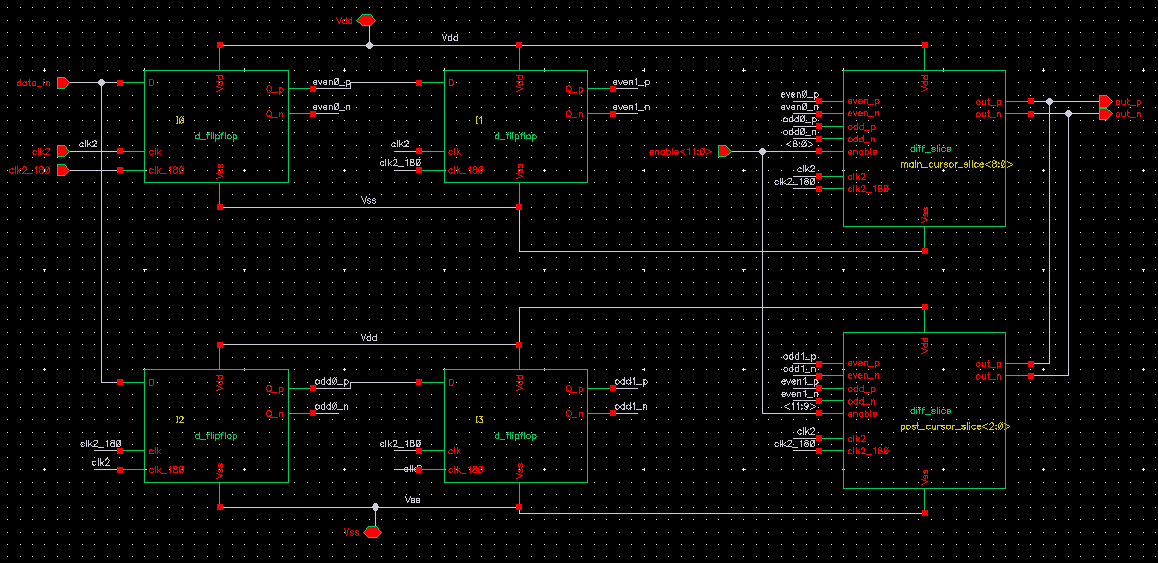
\includegraphics[scale=0.25]{img/transmitter.png}}
  \caption{Transmitter top level circuit}
  \label{fig:top_level_tx}
\end{figure}

\begin{figure}[H]
  \centering
  {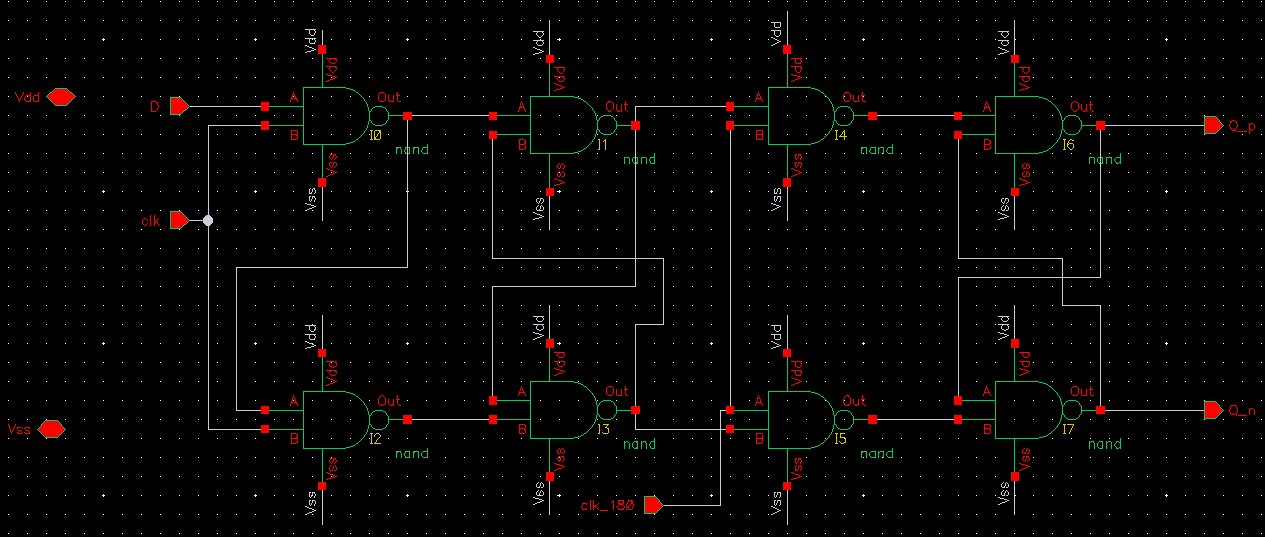
\includegraphics[scale=0.47]{img/flipflop.png}}
  \caption{D-Flipflop}
  \label{fig:flipflop}
\end{figure}

\begin{figure}[H]
  \centering
  \subfigure[Differential slice]
  {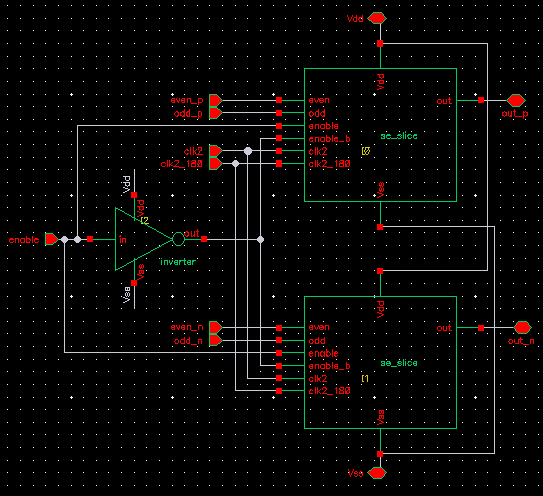
\includegraphics[scale=0.6]{img/diff_slice.png}}
  \subfigure[Single-ended slice]
  {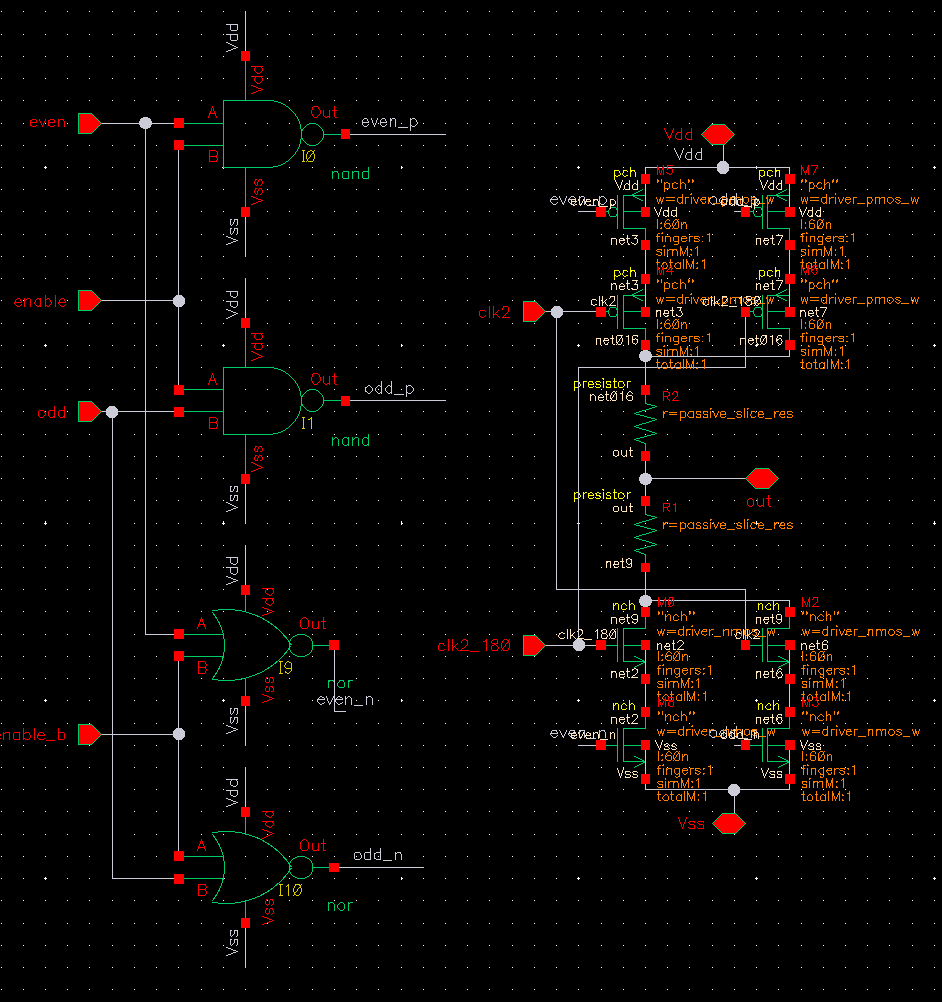
\includegraphics[scale=0.5]{img/se_slice.png}}
  \caption{Slice circuits}
  \label{fig:slices}
\end{figure}


\begin{figure}[H]
  \centering
  \subfigure[Inverter]
  {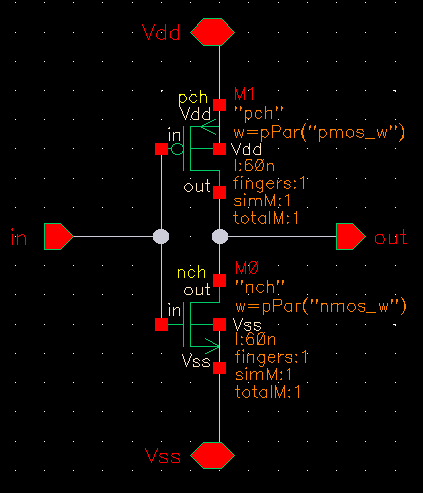
\includegraphics[scale=0.5]{img/inverter.png}}
  \subfigure[NAND gate]
  {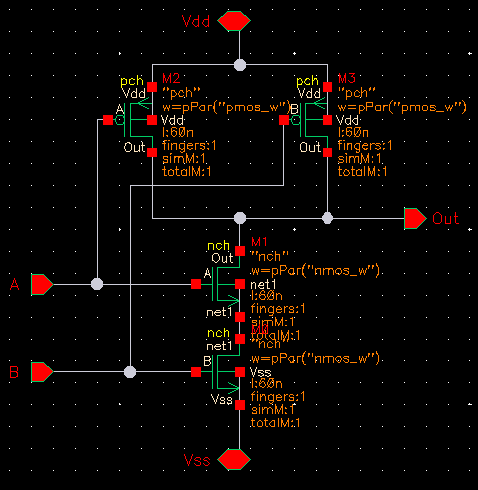
\includegraphics[scale=0.5]{img/nand.png}}
  \subfigure[NOR gate]
  {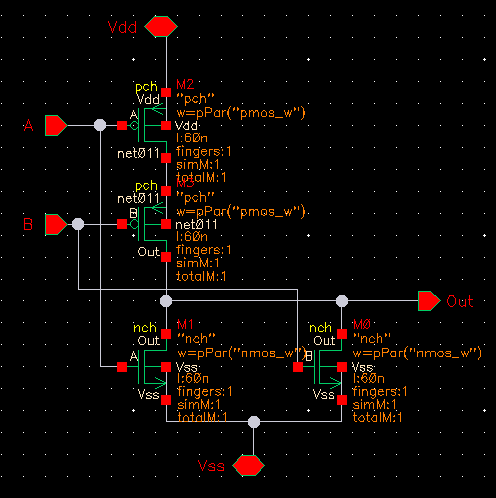
\includegraphics[scale=0.5]{img/nor.png}}
  \caption{Simple gate circuits}
  \label{fig:gates}
\end{figure}